\section{Future Work}
\label{sec:future}
The project code in its current form have a number of shortcomings that should
be improved in order to increase usability.
%These shortcomings and suggestions
%are presented here in a list that is loosely sorted after how critical or usable
%an correction/addition is.

\subsection{Use Generic Mesh Interface}
The prototype of the plugin does not use the generic mesh interface from the
design. In order to test a new mesh structure, the user would have to rewrite the
simulator instead of using time on the actual structure. If the plugin was
rewritten to use the mesh interface, it could help save time for the user.

\subsection{Save visMesh-Node Internal State}
Currently, saving the Maya scene will only save the visMesh node by its id and
its visible plugs. This means the simulation settings will be preserved, but the internal
mesh store, the actual simulation, will be deleted when Maya is closed. In order
to save the meshes, the mesh store should be converted into a node attribute that holds
a number of \texttt{MPxData} nodes. This means same routines that save the
simulation parameters will also save the mesh data. In order to do this, a
class/node that is derived from \texttt{MPxData} will have to be created. This
node can then instruct Maya on how to save/load the mesh by overriding any of
the \texttt{writeBinary}, \texttt{writeASCII}, \texttt{readBinary} or
\texttt{readASCII} methods.

Implementing this feature would allow for visualizations of simulations
performed earlier essentially allowing the visualization of a simulation without
using the simulator.

\subsection{Better Plug Types}
Currently, the only plug type that visMesh node accepts is floating point
numbers. This should be changed to allow for more fitting types, if a simulation
only need to take integer arguments, there is no reason to force a float
conversion. Another useful type would be the ability to take other strings than
the init-file as input. This would for instance allow the user to supply the
simulator with a clean directory it could use for temporary files or to save its
own state based on how many ticks it have done.

\subsection{UI Button to Add the Mesh}
In order to integrate better with the Maya environment the plugin could add a
button to Mayas own UI so the visMesh node can be added with a single click
instead of running the MEL script from Section \ref{sec:melsetup}.

This addition to the UI should be done in the plugins registration phase (during
\texttt{initializePlugin} and should be done through Mayas \textit{QT}
implementation.

\subsection{Support Animated Parameters}
Plugs in Maya are animatable, which means that, for instance, a ``step length''
parameter can be set to change over time. A usage example is if you have a
simulation where you know that only very little details is required in the first
part of the situation, but it will be very useful later on, being able to
animate the step size will help. In the current visMesh plugin, it is possible
to animate the plug itself, but it will cause the plugin to reset the simulation
every time a parameter change.

\subsection{Better/tidier CMake File}
Currently the CMake file contains absolute paths for libraries such as the
BLAS\footnote{Needed to compile/link DSC}-, Chan-Vese- and DSC libraries. A
cleaner CMake file would make it easier for future users to pick it up and add
work to it.

\subsection{Proper Code Documentation}
Currently the code is only documented by this report and a few comments in the
code files themselves. While this may suffice for now, if the projects codebase
grows, it might be advisable to add proper documentation for each function and
perhaps start using a documentation generator like Doxygen\footnote{
\myurl{http://www.stack.nl/~dimitri/doxygen/}} to generate proper overviews of
the classes/methods.

\subsection{Avoid Redundant Vertices}
When vertex data are drawn from the simulator the plugin will not spot vertices
that have been added before, so if a simulator sends the same vertex twice, it
will be stored twice. This can be avoided if a labelling scheme is implemented,
reducing the memory footprint.

\begin{figure}
        \centering
        \begin{subfigure}[b]{0.48\textwidth}
                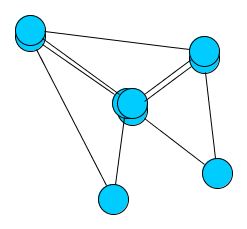
\includegraphics[width=\textwidth]{img/vertex_overlay0.png}
                \caption{3 polygons that share different points put store them
                with individual vertices, not that the bundled up vertices would
                normally be in exactly the same spot, they're staggered for
                illustrative purposes.}
                \label{fig:vertex-overlay0}
        \end{subfigure}%
        \hspace{10px} % use \qquad??
        \begin{subfigure}[b]{0.48\textwidth}
                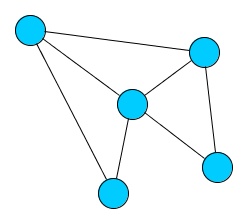
\includegraphics[width=\textwidth]{img/vertex_overlay1.png}
                \caption{3 polygons sharing points that also share vertices,
                this stores the same geometry with four less vertices.}
                \label{fig:vertex-overlay1}
        \end{subfigure}
        \caption{The current (left) and the proposed(right) way of storing the
        triangle mesh by sharing vertices.}
        \label{fig:vertex-overlay}
\end{figure}

Figure \ref{fig:vertex-overlay} demonstrates this point with a simple triangle
mesh, where the current method would store nine vertices and nine edges, the optimum
way for storing the mesh would only store five vertices and seven edges. In small
meshes like this example, there is not much to be gained, but the overhead in
storing redundant vertices increases with the mesh complexity.